\chapter{Introduction}
\label{c:intro}

\note{Introductory text goes here!}

%\date{\today}

%\documentclass[12pt]{article}
% TODO unccoment this
% \documentclass[10pt]{article}


%\usepackage{url}
%\usepackage{hyperref}
%\usepackage[authordate,backend=biber,autolang=none,booklongxref=false,%
%bibencoding=utf-8,strict,%
%annotation]{biblatex-chicago}
%\usepackage{graphicx}
%\usepackage[section]{placeins}
%\usepackage{fontspec}
%\usepackage[shortcuts]{extdash}
%\usepackage{dsfont}
%\usepackage{amsmath}

%\setmainfont[Ligatures=TeX]{Linux Libertine O}

% TODO uncomment this
%\setmainfont[Ligatures=TeX]{Arial}

%\addbibresource{main.bib}
%\addbibresource[datatype=ris]{irizarry.bib}

%\setlength{\parindent}{0em}
%\setlength{\parskip}{1em}

%\usepackage{mathtools}
%\newcommand\givenbase[1][]{\:#1\lvert\:}
%\let\given\givenbase
%\newcommand\sgiven{\givenbase[\delimsize]}
%\DeclarePairedDelimiterX\Basics[1](){\let\given\sgiven #1}

%\begin{document}

%\maketitle

\section{Omics}

\subsection{Introduction to Omics}

Encyclopædia Britannica \parencite[Bioinformatics]{Lesk2016} identifies the following fields of study bearing the ``\=/omics'' suffix:
\begin{itemize}
\item genomics -- ``[the] study of the structure, function, and inheritance of the genome (entire set of genetic material) of an organism'' \parencite[Genomics]{Griffiths2016}.
\item proteomics -- ``[the study of] the distribution of proteins in cells'' \parencite[Bioinformatics]{Lesk2016}.
\item metabolomics -- ``[the study of] the nature and traffic patterns of transformations of small molecules by the biochemical pathways active in cells'' \parencite[Bioinformatics]{Lesk2016}.
\item interactomics -- ``[the study of] the patterns of protein-protein and protein–nucleic acid interactions'' \parencite[Bioinformatics]{Lesk2016}.
\item transcriptomics -- ``[the study of] the pattern of RNA synthesis from DNA'' \parencite[Bioinformatics]{Lesk2016}.
\item pharmacogenomics, metagenomics and metaproteomics.
\end{itemize}

This list of the ``omics fields'', as given by the \textit{Encylopædia} is not complete, nor could it be. It doesn't for example include lipidomics, which \textcite{Wenk2005} defines as ``systems-level analysis of lipids and factors that interact with lipids''. The reason for this lack of completeness is the \textit{rate of change} of the ``omics'' fields. New ways of obtaining large quantities of data about living organisms are continuously discovered, while the accuracy, cost and feasibility of the old techniques is improved.

\subsection{Rapid Evolution of Omics}

\begin{figure}[ht] \label{microVsSeq}
	\centering
	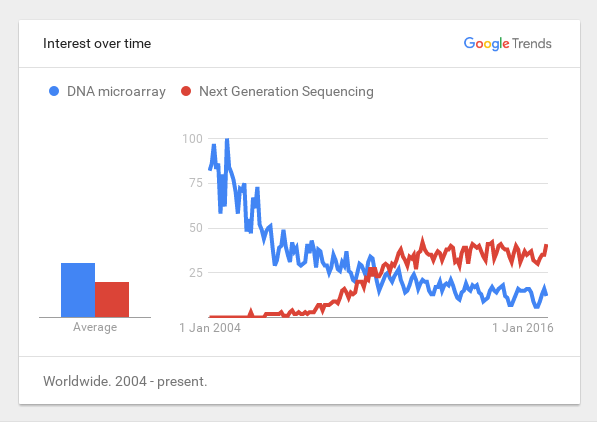
\includegraphics[width=135mm]{MicroarrayVSSequencing.png}
	\caption{Relative popularity of search terms involving ``DNA Microarray'' and ``Next Generation Sequencing'' keywords. Courtesy of Google Trends.}
\end{figure}


A good example at the time of the writing is a shift from an established technique of DNA/RNA Microarray Analysis to the so-called Next Generation Sequencing \parencite{Mardis2008}. This shift is captured by \textcite{GoogleTrends}, Fig. \ref{microVsSeq}. As one can see google searches involving ``DNA microarray'' keywords are in constant decline since 2004, whereas google searches involving ``Next Generation Sequencing'' are on the rise, overtaking ``DNA microarray'' around 2009, about a year after the paper of \textcite{Mardis2008}. While this only provides a proxy indicator of the general interest in these two topics, it does neatly illustrate how Next Generation Sequencing has overtaken Microarrays in transcriptomics.

\subsection{Breadth of data gathering techniques in Omics}

The omics fields not only evolve quickly, but also feature significant breadth of techniques involved. Metabolomics for example involves working with Nuclear Magnetic Resonance (NMR), Mass Spectrometry (MS), Raman Spectroscopy (RS) and Infrared Spectroscopy (IR) data \parencite{Madsen2010}. This breadth is further exacerbated by a great variety within each technique. If we look at Mass Spectrometry, in order to perform an analysis one has to choose from one of many types of MS detectors, chromatographs and extraction types. With this amount of choice one quickly gets hundreds, if not thousands of possible sub-techniques.

\subsection{Importance of generic data analysis tools}

With such variety of rapidly evolving techniques involved, a need emerged to develop generic data analysis methods \& techniques, which can be applied to a wide range of omics fields and provide better insights into the nature of objects studied by these fields, be it genes, proteins, metabolites or lipids. Such methods need to cover as many existing data gathering techniques as possible and be resistant to their rapid change.

It appears that Individual Specific Effects (\textbf{ISE}) may be such generic tool. We introduce them with appropriate background in section 
\ref{ISE}

\section{Omics Data analysis}

\subsection{Differentially responding features}

Although data analysis tasks vary from one omics field to another, one of the major data analysis tasks among these is to look at a whole genome, proteome, metabolome, lipidome, etc. and identify the genes, proteins, metabolites, lipids, etc., whose levels change in response to the change in treatment, disease status or other conditions. Borrowing terminology from Machine Learning we can use the word \textbf{feature} as a collective name for genes, proteins, metabolites, lipids, and others alike.

Such analysis, if successful, yields a list of features, which can be given to domain specialists (geneticists, molecular biologists, pharmacologists) for further analysis.

There is no universally agreed criteria, by which one can distinguish differentially responding features from non-differentailly responding features. Some common practice is however widely accepted. In the context of microarray analysis:
\begin{enumerate}
    \item One should pre-process raw data. This pre-processing should include:
    \begin{enumerate}
        \item Removing from consideration data points, whose signal is not significantly greater than background noise \parencite{Smyth2004}
        \item Accounting for systematic bias, which results from physical constraints of the experimental technique, like geometry of the microarray, change in temperature in the laboratory between running subsequent experiments, and even damage due to atmospheric ozone \parencite{Fare2003}. This process is known as normalisation \parencite{Wit2004}.
    \end{enumerate}
    \item One can use General Linear Models (GLMs) and corresponding t-statistic, F-statistic, B-statistic or fold change to order features according to the likelihood of differential response to treatment. \parencite{Smyth2004}
    \item One has to account for the multiplicity effect, which results from considering thousands or millions of data points at once \parencite{Wit2004} We discuss possible measures to account for this effect in the next subsection.
\end{enumerate}

\subsection{False Discovery Rate} \label{FDR}

Let us consider a collection of features $$x_{1}, \ldots, x_{n}$$ where $n$ is the number of features under consideration. Depending on the experimental technique, the magnitude of $n$ can vary from about $10^{3}$ to about $10^{6}$.

For each feature $x_{i}$ let us collect intensity measurements $$M_{i,1}, \ldots, M_{i,k}$$ where k is the number of individuals under investigation and $$(m_{i,1}, \ldots m_{i,k})$$ are the measured values. For each feature $x_{i}$ let us define a null hypothesis $N_{i}$, which states that $x_{i}$ does not respond differentially to the changes in treatment. Once we have decided on appropriate statistic $$T(M_{i,1}, \ldots M_{i,k})$$ which captures the notion of ``differential response'', we can define a p-value $p_{i}$ as the probability of observing the same, or more extreme value of the statistic under $N_{i}$, i.e.  $$p_{i}=\mathds{P}(T(m_{i,1}, \ldots m_{i,k}) \geq T(m_{i,1}, \ldots m_{i,k}) \given N_{i})$$

Such value is useful, because the lower it is the more confidently we can say that $N_{i}$ is false, i.e. the feature $x_{i}$ responds differentially to the change in treatment. It is customary to reject $N_{i}$ if $p \leq 0.05$. In the omics setting however, assuming such threshold of 0.05 would lead to artificially high number of incorrectly rejected $N_{i}$ or ``False Discoveries''. Let $R$ be the number of of hypotheses rejected, and let $V$ be the number of true hypotheses incorrectly rejected. $R$ is an observable random variable, whereas $V$ is unobservable. \textcite{Benjamini1995} call $\mathbf{E}(V/R)$ False Discovery Rate (FDR) and give a procedure for controlling it. Before we look into their procedure, let us show why it is necessary.

Let us assume that all of $N_{i}$ are true and we compute p-values $p_{i}$ as described above, and reject any $p_{i} \leq 0.05$. Then $V = R$ and we have $$V \sim \operatorname{Binomial}(n, 0.05)$$ which leads us to $$\mathbf{E}(V)=0.05n$$which under our previous assumptions on the size of $n$ gives us between about $10^{2}$ to $10^{5}$ false discoveries, and in fact, a FDR of $1$.

While the example above gives perhaps unrealistic worst-case scenario with $0$ true discoveries to be made, it hopefully shows why rejecting $N_{i}$ with no multiplicity correction is inappropriate.
\subsubsection{Benjamini-Hochberg procedure}
Without loss of generality, let us assume that the sequence $p=\{p_{i}\}$ is non-decreasing. Let $c$ be a sequence of corrected p-values $$c=\{\frac{p_{i} \times n}{i}\}$$Let k be the largest index such that $c_{k} \leq q$, where $q$ is an arbitrary threshold, e.g. 0.05. \textcite{Benjamini1995} show that if we reject all $$N_{1}, \ldots, N_{k}$$
we have that $$\mathbf{E}(V/R) \leq q$$In a study with large number of hypotheses $n$ a researcher using the Benjamini-Hochberg procedure will be expected to make $(1-q)\times 100\%$ true discoveries.

\subsection{Omics Analysis in Practice}

A bioinformatician will usually use an existing implementation of the techniques described above. There are several libraries and software packages available for omics analyses. Two have been evaluated for this literature review and were used in obtaining preliminary results.

\subsubsection{Bioconductor}

Bioconductor is a collection of software packages for R programming language, which implements tools for analysis and comprehension of genomic data \parencite{Huber2017}. Bioconductor contains over 1296 packages \parencite{Bioconductor}. It is open-source, and developed by a diverse community of users. Although the scope and quality of packages distributed as part of Bioconductor varies, some of its packages are notable for being both applicable to a wide array of data gathering techniques and of high quality. One of such packages is Limma, which allows for analysis of microarray data, and is discussed separately. R \& Bioconductor are popular in the biostatistical community.

\subsubsection{Limma}

Limma is a software package, distributed as part of Bioconductor. It addresses the problem of identifying differentially expressed genes in microarray experiments \parencite{Smyth2004}, and, in combination with other Bioconductor packages, in RNA-Seq experiments \parencite{Law2016}. Limma allows users to define a ``design matrix'', which is used to fully specify an experiment-dependent General Linear Model (GLM). The GLM is then subsequently fitted to expression data of each gene separately. Limma uses empirical Bayes to robustly estimate the parameters of the fit, even when the number of microarrays is small \parencite{Smyth2004}.

\subsubsection{Biopython}

Biopython is a software library, which partially overlaps, but mostly complements the functionality of Bioconductor. It is likewise open-source, but it's written in Python programming language and is popular in the bioinformatics community. Biopython's main strength is working with biological sequences, and it allows for a range of sequence manipulation operations, such as two sequence alignment, multiple sequence alignment, sequence assembly, translation of RNA \symbol{8594} DNA sequences, as well as connects to multiple online databases, such as the NCBI Entrez Utilities, ExPASy, InterPro, KEGG and SCOP.Bio.Blast \parencite{Cock2009}. Biopython also includes some rudimentary support for working with microarray data \parencite{Zuzan2004,Kurkiewicz2016}, but this support lacks the sophistication and capability of Biconductor and Limma.

\section{Individual Specific Effects} \label{ISE}

Let us go back to the notation from section \ref{FDR}. Let $$x_{1}, \ldots, x_{n}$$ be a collection of features, and let us have a sequence of measurements for each feature
$$M^{k}_{i}=\{M_{i,1}, \ldots, M_{i,k}\}$$
where k is the number of individuals under investigation. Each $M_{k, j}$ is a measurable random variable. Let $$p=\{p_{i}\}$$ be a sequence of p-values as defined in section \ref{FDR}, and again let us assume, without loss of generality, that this sequence is non-decreasing. If necessary, we may have to reorder $x_{i}, M_{i}^{k}$ and $m_{i}^{k}$ to correspond to the non-decreasing order of p-values.

Further, let $D=\{D_{1}, \ldots, D_{j}, \ldots, D_{k}\}$ be a sequence of measurements of the disease severity or treatment dose of individual $j$, where greater $D_{j}$ signifies more advanced disease or higher dose of treatment. Each $D_{j}$ is a measurable random variable, and each $D_{j}$ corresponds to the set of feature intensities $$\{M_{i,j} | 1 \leq i \leq n \}$$.

Let us now fit a simple regression model to each $(D_{j}, M^{i}_{j})$. For each fit $(D_{j}, M^{i}_{j})$, let $$\epsilon_{i, 1}, \ldots, \epsilon_{i, k}$$ be the residual, i.e. the difference between $m_{i, j}$ and a value predicted from the regression model. We can now define Disease Specific Effect $DSE^{j}_{l}$, for any individual $j$ and any $l \leq n$ as such
$$DSE^{l}_{j}=\sum^{u=l}_{u=1}(\epsilon_{u,j})$$
In other words $DSE^{l}_{j}$ is a sum of l residuals corresponding to the l lowest p-values $p_{1}, \ldots, p_{l}$.

If we set $l = n$, then we call $DSE^{l}_{j}$ and Indvidual Specific Effect of indvidual $j$, and write it $ISE_{j}$. Both Disease and Individual Specific Effect are measurable random variables.

It is conjectured that by accounting for either some of the DSEs or the ISE for each individual can allow us to better identify deferentially responding features.

The procedure of accounting for any $DSE^{l}_{j}$ is as follows: for any $M^{i}_{j}$ we compute a simple linear regression model to each $(D_{j}, M^{i}_{j} - DSE^{l}_{j})$ and we compute p-values as in section \ref{FDR}. Preliminary results show that applying this procedure allows us to increase the number of correctly rejected $N_{i}$.
%\printbibliography
%\end{document}
\section{Thesis Statement}
\label{c:intro:thesisstatement}

\input{"10-introduction/thesis_statement.tex"}
